\chapter{Needle Model}
\label{sec:needlemodel} % Always give a unique label
% use \chaptermark{}
% to alter or adjust the chapter heading in the running head

The needle model presented in this thesis is based on minimizing the bending energy in the needle, which is represented as a beam and characterized as a parametric polynomial curve. Other existing needle modeling approaches account for bending energy, generally to determine the equilibrium state between the needle and the surrounding elastically-deformed tissue\cite{roesthuis_modeling_2015, misra_mechanics_2010, abayazid_integrating_2013}.

The model is initialized with the mechanical properties of the needle and updated throughout insertion with the most recent pose of the needle base and the latest observed points on the needle shaft. This allows estimation of the shape of the needle using only a few new images without requiring an explicit model of the forces acting on the needle.

Mechanics-based models make restrictive assumptions about the trajectory of the needle by limiting the number bends in the needle shaft\cite{abayazid_integrating_2013}. Models that assume a single direction of insertion preclude the trajectories achievable with highly-flexible needles. By parameterizing the needle coordinates independently of the insertion direction or depth, this model can represent needles inserted in any direction relative to the scanner coordinate frame.

Both nonholonomic kinematic models and mechanics-based beam bending models require extensive characterization of the properties of the needle and the tissue in order to accurately account for the tip and shaft loads placed on the needle. Tissue properties vary between tissue types and patients, and characterization of properties to the extent required by these models would probably not be possible to accomplish during a procedure. In contrast, this model does not require characterization of mechanical properties, since the constraints imposed on the needle by its interaction with surrounding tissue are measured through the observed shape of the needle.

In the context of MRI, it would be very time-consuming to exactly evaluate the state of the needle using only observations from imaging. The core idea of this model is to take a few observations and then optimize a model that meets those constraints and the constraints imposed by the mechanics of the needle. Provided that the constraints are carefully chosen, the needle model will be "close enough" to the actual state of the needle from the perspective of guiding insertion and planning future imagery.

\section{Assumptions}
\begin{itemize}
\item As currently formulated, this model only considers straight needles with uniform stiffness and cross-section.

\item Actuated devices such as flexible-tip needles and continuum robots are not considered.

\item The state of the needle can be observed in imaging.

\end{itemize}

The model uses the following information about the composition and state of the needle:
\begin{itemize}
\item 6-degree-of-freedom pose of the base of the needle, via the forward kinematics of the insertion robot
\item Length of the needle
\item Diameter of the needle
\item Elastic modulus of the needle
\item Multiple observed coordinates on the needle shaft from a sparse set of cross-sectional images
\end{itemize}

\begin{tabular}{@{}ll@{}} 
\textbf{Symbol} & \textbf{Description} \\
$U_B$ & mechanical bending energy \\
$L$ & needle length \\
$r$ & needle radius \\
$s$ & parametric variable \\
$n$ & polynomial degree \\
$\delta$ & needle tip offset \\
$\rho$ & needle curvature \\
$\kappa$ & needle error weight \\
$k$ & observation index \\
$E$ & elastic modulus \\
$I$ & second area moment of inertia \\
$x \in X$ & \textbf{X-component}, set of X-components of needle coordinate \\
$y \in Y$ & \textbf{Y-component}, set of Y-components of needle coordinate \\
$z \in Z$ & \textbf{Z-component}, set of Z-components of needle coordinate \\
$v $ & magnitude of deflection relative to the needle neutral axis \\
$\textbf{V}$ & vector, needle coordinate \\

$C$ & cumulative cost of the needle model configuration \\
$\textbf{V}$ & vector, needle coordinate \\

\end{tabular}

\section{Beam Bending Energy}
The actual biopsy needle contains several parts with different mechanical properties, such as an inner rod that sides within an outer shell. Since these interactions are computationally expensive to model exactly and unnecessary to account for unless a very high degree of fidelity is desired, the model presented here simplifies the needle as a solid cylindrical beam and neglects the change in cross-sectional area at the needle tip. Under these assumptions the area moment of inertia of the needle in cross-section is constant along its entire length and can be written as Equation \ref{eq:beam_inertia}. 

\begin{equation}
\label{eq:beam_inertia}
I = \frac{\pi}{4}r^4
\end{equation}


Since the needle is assumed to have a constant diameter along its entire length, it can be represented as an Euler-Bernoulli beam with constant cross-sectional area. The transverse bending energy in a straight beam with constant cross-section, shown in Equation \ref{eq:bending_energy_transverse}, is a function of the curvature in the beam integrated over its length. Equation \ref{eq:curvature} shows the calculation of curvature in an arc.

\begin{equation}
\label{eq:bending_energy_transverse}
U_B = \frac{EI}{2}\int_{0}^{L}\frac{1}{\rho^2}dl
\end{equation}

\begin{equation}
\label{eq:curvature}
\frac{1}{\rho} = \frac{d^2v/dl^2}{(1+(dv/dl)^2)^{3/2}} \simeq \frac{d^2v}{dl^2}
\end{equation}

In a beam subject to zero load its cumulative curvature is zero, so its total bending energy is also zero. Higher curvatures correspond to sharper bends, which means that a beam that is predominately straight with one very sharp bend will have a greater bending energy than a beam of the same length where the bend is gentle and distributed along its entire length. Beams adopt shapes that minimize their cumulative bending energy while meeting constraints imposed by external fixtures.


\section{Parametric Polynomial Space Curves}
The needle curve is represented using an $n$-degree parametric polynomial function, shown in Equation \ref{eq:parametric_curve}.

% The first derivative of this polynomial is shown in Equation \ref{eq:parametric_curve_d}.

In the context of representing a needle, $n$ represents the maximum number of inflection points in each axis. A needle inserted without rotation would deflect consistently in one direction and its shape could be represented using at minimum a 3rd-degree polynomial ($n=3$).

\begin{equation}
\label{eq:curve_vector}
\textbf{V}=\begin{bmatrix}x(s) \\ y(s) \\ z(s) \end{bmatrix}
 \end{equation}

\begin{equation}
\label{eq:parametric_curve}
\begin{cases} x(s) = a_n s^n + a_{n-1} s^{n-1} + ... + a_1 s + a_0 \\
 y(s) = b_n s^n + b_{n-1} s^{n-1} + ... + b_1 s + b_0  \\
 z(s) = c_n s^n + c_{n-1} s^{n-1} + ... + c_1 s + c_0 \end{cases} \\
 s\in (0, 1)
 \end{equation}
 
%  \begin{equation}
% \label{eq:parametric_curve_d}
% \begin{cases} \frac{dx}{ds} = n a_n s^{n-1} + (n-1) a_{n-1} s^{n-2} + ... + a_1\\
%  \frac{dy}{ds} = n b_n s^{n-1} + (n-1) b_{n-1} s^{n-2} + ... + b_1  \\
%  \frac{dz}{ds} = n c_n s^{n-1} + (n-1) c_{n-1} s^{n-2} + ... + c_1 \end{cases} \\
%  s\in (0, 1)
%  \end{equation}

The three spatial coordinates $x$, $y$, and $z$ are functions of a unitless parameter $s$, which ranges from 0 at the needle base to 1 at the needle tip. Given sets of needle coordinates $X$, $Y$, and $Z$, the relationship between the values of $s$ and the positions of the needle coordinates is established by the distances between the needle coordinates, calculated in Equation \ref{eq:distance}, and the proportion of each distance to the cumulative distance between all the coordinates, calculate in Equation \ref{eq:parameter}.

\begin{equation}
\label{eq:distance}
\begin{cases}
d_k = 0 &\mbox{if } k=0 \\
d_k = \sqrt[]{(X_k - X_{k-1})^2 + (Y_k - Y_{k-1})^2 + (Z_k - Z_{k-1})^2} &\mbox{if } k>0
\end{cases}
\end{equation}

\begin{equation}
\label{eq:parameter}
\begin{cases}
s_k = 0 &\mbox{if } k=0 \\
s_k = s_{k-1} + \frac{d_k}{L_needle}&\mbox{if } k>0
\end{cases}
\end{equation}

While an alternative implementation could represent the $x$- and $y$-components of the coordinate as a function of the $z$-component, using an independent parameter allows the curve to represent torturous trajectories without placing restrictions on the direction of needle insertion.

The maximum number of inflection points in each axis, and consequently the maximum number of changes in needle direction that the curve can represent, is limited by the degree of the polynomial.

\section{Curve Fitting}
The purpose of curve fitting is to choose coefficients of the parametric function in Equation \ref{eq:parametric_curve} given a number of observed needle cross section coordinates so that the total bending energy in the curve and the error between the curve and the needle coordinates are minimized.

Prior to optimization, initial coefficients for each curve are found by fitting a polynomial of degree $n$ to the needle coordinates using least-squares. While this initial solution is not representative of the actual mechanical factors that determine the shape of the needle, it approximates the minimum bending energy curve and helps prevent the optimization for reaching a local minimum or other failure condition.

The curve is optimized to minimize bending energy using Sequential Least SQuares Programming (SLSQP), which is an iterative constrained Non-Linear Programming (NLP) search algorithm\cite{kraft_software_1988}.

\subsection{Cost Function}
The cost function subject to minimization is shown in Equation \ref{eq:cost_function}. It is a modification of Equation \ref{eq:bending_energy_transverse} which adds the weighted mean error between the needle coordinates and the nearest point on the curve. Since the elastic modulus and area moment of inertia are constant along the length of a straight needle with uniform cross-section, they could be omitted in this calculation. 

TODO: (Fu) Update cost function with correct labeling

TODO: (Fu) Add additional constraint option for overall error

\begin{equation}
\label{eq:cost_function}
% C = \kappa \sum_{i=0}^k \epsilon_i + \frac{EI}{2}\int_{0}^{L}\frac{1}{\rho^2}dl
C = \frac{EI}{2} \int_{0}^{L} \frac{1}{\rho^2}dl
\end{equation}

While equality constraints can also be used to guide the optimized curve to intersect all the needle coordinates, this approach risks over-constraining the curve where the degree of the polynomial is close to the number of equality constraints.

% \subsection{Slope Constraints}
% The SLSQP optimization is constrained so the curve is tangential to the insertion vector at the needle entry point.

% \begin{equation}
% \label{eq:slope_constraint_y}
% \frac{dy}{dx}(t_{entry}) = orientation_{entry,y}
% \end{equation}

% \begin{equation}
% \label{eq:slope_constraint_z}
% \frac{dz}{dx}(t_{entry}) = orientation_{entry,z}
% \end{equation}
\subsection{Constraints}
The optimization is constrained by Equation \ref{eq:base_position_constraint} such that the coordinates of the curve at t=0 matches the position of the base of the needle.
% \begin{equation}
% \label{eq:base_position_constraint}
% \begin{cases} X_{k=0} = a_0 \\
%  Y_{k=0} = b_0  \\
%  Z_{k=0} = c_0 \end{cases}
%  \end{equation}
 
 \begin{equation}
 \label{eq:base_position_constraint}
 \textbf{V}_{k=0}=\begin{bmatrix} a_0 \\ b_0 \\ c_0 \end{bmatrix}
 \end{equation}

The optimization is also constrained by Equation \ref{eq:length_constraint} so that the length of the curve between \textit{t}=0 and \textit{t}=1 is equal to the length of the needle.

\begin{equation}
\label{eq:length_constraint}
L = \int_0^1 \sqrt[]{\frac{dx}{ds}^2 + \frac{dy}{ds}^2 + \frac{dz}{ds}^2} d\tau
\end{equation}

\begin{equation}
\label{eq:rsme_constraint}
\epsilon \geq \sqrt[]{\frac{\sum_{i=0}^{k}(V_i - V_{i, obs})^2}{k}}
\end{equation}

\begin{equation}
\label{eq:length_calculation}
L = \int_0^\tau \sqrt[]{\frac{dx(\tau)}{ds}^2 + \frac{dy(\tau)}{ds}^2 + \frac{dz(\tau)}{ds}^2} d\tau
\end{equation}

% \begin{equation}
% \label{eq:length_constraint}
% L = \int_0^1 \sqrt[]{\frac{dx(\tau)}{ds}^2 + \frac{dy(\tau)}{ds}^2 + \frac{dz(\tau)}{ds}^2} d\tau
% \end{equation}

% \begin{equation}
% \label{eq:length_calculation}
% L = \int_0^\tau \sqrt[]{\frac{dx(\tau)}{ds}^2 + \frac{dy(\tau)}{ds}^2 + \frac{dz(\tau)}{ds}^2} d\tau
% \end{equation}

\subsection{Assumptions}

TODO: (Fu) "The assumption in 3.3.4 is made but the result is not given any quantitative information. For example, in your experiment setting, “deflection of the needle tip throughout insertion is be comparatively small”, how small should it be? Will this number change when different tissue/material the needle interacts with?"

Equations \ref{eq:distance} and \ref{eq:parameter} assumes that length of the needle model curve is close to the sum of the distances between the sampled points on the needle. This is met if the deflection of the needle tip throughout insertion is be comparatively small and the number of sample points is be sufficient to characterize the shape of the needle.

% \section{Piecewise Polynomial Space Curves}
% There is a practical upper limit on the degree of the polynomial imposed by the regression and optimization function, which means that some needle trajectories cannot be practically represented using a single polynomial. In these cases a piecewise polynomial function can be used, with additional constraints imposed so that the curves are contiguous and continuous at the points of intersection.

% \section{Needle Motion Model}
% The minimum bending energy model provides a reasonable estimation of the pose of the needle tip throughout insertion by modeling the shape of the needle shaft. One way to estimate the needle tip pose after a small insertion is to assume that the tip will move in a straight line from the tip of the needle. This assumes that any curvature will be small enough that the cross section of the needle could be captured in the imaging window.

% - Could also use the kinematic bicycle model to find an offset tip position using the needle base orientation.

\section{Software Implementation}
Algorithm \ref{alg:update_curve_fit} shows the process of calculating polynomial coefficient to minimize bending energy given a set of observed needle coordinates. \ref{fig:curve_fit_flow} shows the flow of data through the curve optimization function. 

\begin{figure}[h]
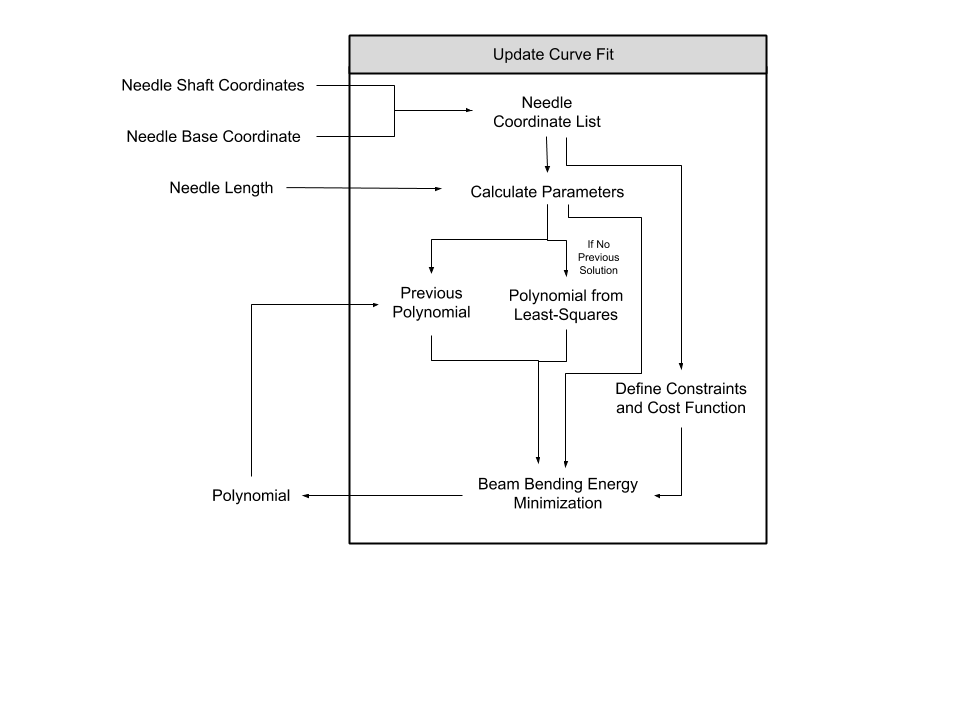
\includegraphics[width=1.0\textwidth]{Fig/chap3/Update_Curve_Fit.png}
\caption{Flowchart for beam optimization function.}
\label{fig:curve_fit_flow}
\end{figure}

\begin{algorithm}
\caption{Curve Optimization}
\label{alg:update_curve_fit}
\begin{algorithmic}[1]
\Procedure{Update Curve Fit}{$coords_{needle},L_{needle},poly_{prev}$}
\State $t \gets CalculateParameters(coords_{needle}, L_{needle})$
\If {$poly_{prev} is None$}
	\State $poly_{init} \gets LeastSquares(coords_{needle})$
\Else
	\State $poly_{init} \gets poly_{prev}$
\EndIf
\State $cons \leftarrow DefineConstraints(t, coords_{needle}, L_{needle})$
\State $poly_{opt} \gets DoOptimization(poly_{init}, cons)$
\State \textbf{return} $poly_{opt}$
\EndProcedure
\end{algorithmic}
\end{algorithm}

\begin{figure}[h]
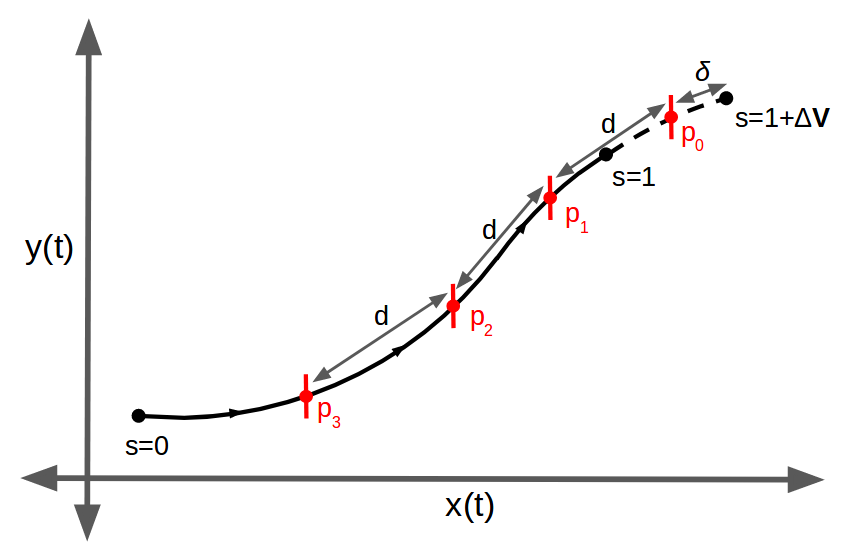
\includegraphics[width=1.0\textwidth]{Fig/chap3/curvefit_pt1.png}
\caption{Given a number of samples, the spacing between the samples, an offset distance from the needle tip, and a new needle base pose, the expected coordinate of the needle is calculated at each sample point.}
\label{fig:curve_fit_pt1}
\end{figure}

\begin{figure}[h]
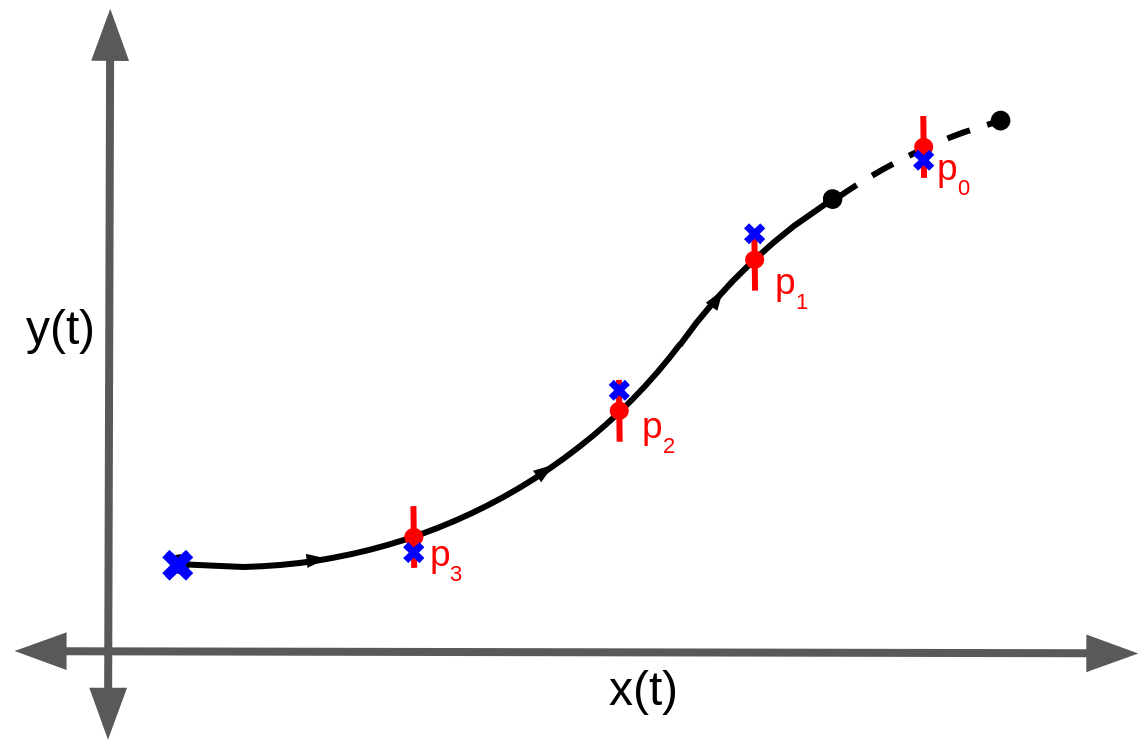
\includegraphics[width=1.0\textwidth]{Fig/chap3/curvefit_pt2.png}
\caption{New imaging is collected at each needle coordinate, and the actual position of the needle is observed.}
\label{fig:curve_fit_pt2}
\end{figure}

\begin{figure}[h]
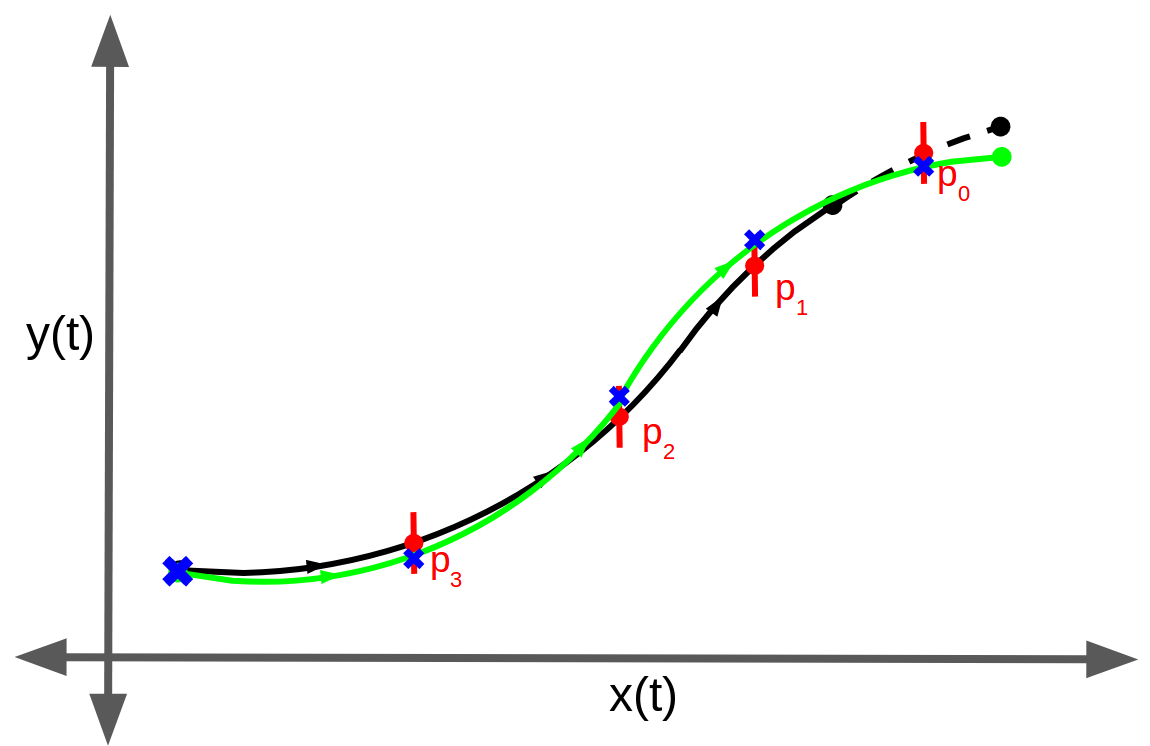
\includegraphics[width=1.0\textwidth]{Fig/chap3/curvefit_pt3.png}
\caption{A new polynomial curve is calculated, optimized to minimize both the cumulative bending energy in the needle and the error between the curve and the observed points.}
\label{fig:curve_fit_pt3}
\end{figure}

